\documentclass[12pt]{article} % 12pt 为字号大小 UTF8
\usepackage{amssymb,amsfonts,amsmath,amsthm}
%\usepackage{fontspec,xltxtra,xunicode}
%\usepackage{times}

%----------
% 定义中文环境
%----------

\usepackage{xeCJK}
\usepackage{color}
% \setCJKmainfont[BoldFont={SimHei},ItalicFont={KaiTi}]{SimSun}
% \setCJKsansfont{SimHei}
% \setCJKfamilyfont{zhsong}{SimSun}
% \setCJKfamilyfont{zhhei}{SimHei}

% \newcommand*{\songti}{\CJKfamily{zhsong}} % 宋体
% \newcommand*{\heiti}{\CJKfamily{zhhei}}   % 黑体


%----------
% 版面设置
%----------
%首段缩进
\usepackage{indentfirst}
\setlength{\parindent}{2em}

%行距
\renewcommand{\baselinestretch}{1.4} % 1.4倍行距

%页边距
\usepackage[a4paper]{geometry}
\geometry{verbose,
	tmargin=3cm,% 上边距
	bmargin=3cm,% 下边距
	lmargin=3cm,% 左边距
	rmargin=3cm % 右边距
}


%----------
% 其他宏包
\usepackage{listings}
\usepackage{subfigure}
%----------
%图形相关
\usepackage[x11names]{xcolor} % must before tikz, x11names defines RoyalBlue3
\usepackage{graphicx}
\usepackage{pstricks,pst-plot,pst-eps}
\usepackage{subfig}
\def\pgfsysdriver{pgfsys-dvipdfmx.def} % put before tikz
\usepackage{tikz}

%原文照排
\usepackage{verbatim}

%网址
\usepackage{url}
\usepackage[framed,numbered,autolinebreaks,useliterate]{mcode}

%----------
% 习题与解答环境
%----------
% %习题环境
% \theoremstyle{definition} 
% \newtheorem{exs}{习题}

% %解答环境
% \ifx\proof\undefined\
% \newenvironment{proof}[1][\protect\proofname]{\par
% \normalfont\topsep6\p@\@plus6\p@\relax
% \trivlist
% \itemindent\parindent
% \item[\hskip\labelsep
% \scshape
% #1]\ignorespaces
% }{%
% \endtrivlist\@endpefalse
% }
% \fi

% \renewcommand{\proofname}{\it{证明}}

%----------
% 我的自定义
%----------

\newcommand{\horrule}[1]{\rule[0.5ex]{\linewidth}{#1}} 	% Horizontal rule

\renewcommand{\refname}{参考文献}
\renewcommand{\abstractname}{\large \bf 摘\quad 要}
\renewcommand{\contentsname}{目录}
\renewcommand{\tablename}{表}
\renewcommand{\figurename}{图}

\setlength{\parskip}{0.4ex} % 段落间距

\usepackage{enumitem}
\setenumerate[1]{itemsep=0pt,partopsep=0pt,parsep=\parskip,topsep=5pt}
\setitemize[1]{itemsep=0.4ex,partopsep=0.4ex,parsep=\parskip,topsep=0.4ex}
\setdescription{itemsep=0pt,partopsep=0pt,parsep=\parskip,topsep=5pt}


%==========
% 正文部分
%==========

\begin{document}
	\title{
		%	{\normalfont\normalsize\textsc{
		%			Xiangtan University  \\[25pt]}}
		\horrule{0.5pt}\\
		\sffamily{数值最优化方法实验报告}
		\horrule{1.8pt}\\[20pt]
	}
	\author{米科润\quad 19信计二班\\201905755824}
	\date{\today} % 若不需要自动插入日期,则去掉前面的注释;{ } 中也可以自定义日期格式
	
	\begin{titlepage}
		\maketitle
		\vspace{30pt}
		\thispagestyle{empty}
	\end{titlepage}
	
	\tableofcontents
	\thispagestyle{empty}
	
	\newpage
	\setcounter{page}{1}
	
	\section{梯度法和信赖域算法的求解}
	\subsection{梯度法}

 	输入:fun,gfun分别是目标函数及其梯度,$x_0$是初始点,epsilon是容许误差。
	
	输出:k是迭代次数,x,val分别是近似最优点和最优值。
	\begin{lstlisting}
	function [k,x,val]=grad(fun,gfun,x0,epsilon)
	maxk=5000; 
	beta=0.5; sigma=0.4;
	k=0;
	while(k<maxk)
		gk=feval(gfun,x0); 
		dk=-gk;
		if(norm(gk)<epsilon), break; end 
		m=0; mk=0;
		while(m<20) 
			if(feval(fun,x0+beta^m*dk)...
				<=feval(fun,x0)+sigma*beta^m*gk'*dk)
				mk=m; break;
			end
			m=m+1;
		end
		x0=x0+beta^mk*dk;
		k=k+1;
	end
	x=x0; val=feval(fun,x0);
	end
	\end{lstlisting}
	
	\subsection{信赖域方法}
	
	$x_0$是初始点,epsilon是容许误差
	
	输出:k是迭代次数,x,val分别是近似极小点和近似极小值。
	
	trustq函数是利用光滑牛顿法求解信赖域子问题的程序
	\begin{lstlisting}
	function [k,x,val] = trustm(x0,epsilon)
	n=length(x0); eta1=0.1; eta2=0.75;
	tau1=0.5; tau2=2.0;
	delta=1; dtabar=2.0;
	x=x0; Bk=Hess(x);k=0;
	while(k<50)
		fk=fun(x);
		gk=gfun(x);
		if(norm(gk)<epsilon)
			break;
		end
		[d,val,lam,i]=trustq(fk,gk,Bk,delta);
		deltaq=fk-val;
		deltaf=fun(x)-fun(x+d);
		rk=deltaf/deltaq;
		if(rk<=eta1)
			delta=tau1*delta;
		else if (rk>=eta2 & norm(d)==delta)
				delta=min(tau2*delta,dtabar);
			else
				delta=delta;
			end
		end
		if(rk>eta1)
			x=x+d;
			Bk=Hess(x);
		end
		k=k+1;
	end
	val=fun(x);
	end
	\end{lstlisting}
	\subsection{问题求解}
	\begin{gather*}
	min\quad f(x)=(x_1-2)^4+(x_1-2x_2)^2\\
	x_0=(0,3)^T
	\end{gather*}
	
	答:
	编写目标函数fun.m、梯度gfun.m、Hess阵Hess.m三个文件
	\begin{lstlisting}
	%目标函数
	function f=fun(x)
	f=(x(1)-2)^4+(x(1)-2*x(2))^2;
	end
	%梯度
	function gf=gfun(x)
	gf=[4*(x(1)-2)^3+2*(x(1)-2*x(2));
		-4*(x(1)-2*x(2))];
	end
	%Hesse阵
	function He=Hess(x)
	He=[12*(x(1)-2)^2+2  -4;
		-4  8];
	end
	\end{lstlisting}
	
	\begin{itemize}
		\item 调用梯度法
		\begin{lstlisting}
	>> x0=[0;3];
	>> [k,x,val]=grad('fun','gfun',x0,1e-5)
		\end{lstlisting}
	
		结果如下图:	
		\begin{figure}[ht]
		\centering
		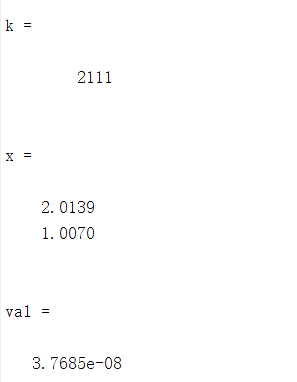
\includegraphics[width=0.4\textwidth]{q1grad.png}
		\caption{question1:梯度法结果}
		\label{fig:fig1}
		\end{figure}
		
		\item 调用信赖域算法
		\begin{lstlisting}
	>> x0=[0.0,3.0];epsilon=1e-5;
	>> [k,x,val] = trustm(x0,epsilon)
		\end{lstlisting}
	
		结果如下图:
		\begin{figure}[ht]
			\centering
			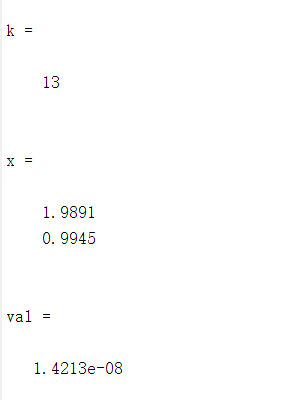
\includegraphics[width=0.4\textwidth]{q1trustq.png}
			\caption{question1:信赖域算法结果}
			\label{fig:fig1}
		\end{figure}
	\end{itemize}

	\section{基本牛顿法的求解}
	基本牛顿法程序:
	
	输入:fun,gfun,Hess分别是目标函数及其梯度和Hess阵,x0是初始点,epsilon为容许误差。
	
	输出:k是迭代次数,x,val分别是近似最优点和最优值。
	\begin{lstlisting}
	function [k,x,val]=dampnm(fun,gfun,Hess,x0,epsilon)
	maxk=5000; 
	beta=0.5; sigma=0.4; k=0;
	while(k<maxk)
		gk=feval(gfun,x0); 
		Gk=feval(Hess,x0); 
		dk=-Gk\gk; 
		if(norm(gk)<epsilon), break; end 
			m=0; mk=0;
		while(m<20) 
			if(feval(fun,x0+beta^m*dk)...
				<=feval(fun,x0)+sigma*beta^m*gk'*dk)
				mk=m; break;
			end
			m=m+1;
		end
		x0=x0+beta^m*dk; k=k+1;
	end
	x=x0;
	val=feval(fun,x);
	end
	\end{lstlisting}
	
	求解问题
	\begin{gather*}
	min\quad f(x)=0.5x_1^2(\frac{x_1^2}{6}+1)+x_2arctanx_2-0.5ln(x^2+1)\\
	x_0=(1,0.7)^T\\
	or\\
	x_0=(1,2)^T
	\end{gather*}

	建立目标函数fun.m,梯度gfun.m,Hesse阵Hess.m函数
	\begin{lstlisting}
	%目标函数
	function f=fun(x)
	f=0.5*x(1)^2*((x(1)^2)/6+1)+x(2)*atan(x(2))-0.5*log(x(2)^2+1);
	end
	%梯度
	function gf=gfun(x)
	gf=[(x(1)^3)/3+x(1);atan(x(2))];
	end
	%Hesse阵
	function He=Hess(x)
	He=[x(1)^2 + 1,0;
	0,1/(x(2)^2 + 1)];
	end
	\end{lstlisting}

	调用基本牛顿法:
	\begin{lstlisting}
	>> x0=[1,0.7];
	>> x1=[1,2];
	>> [k,x,val]=dampnm('fun','gfun','Hess',x0,1e-5)
	>> [k,x,val]=dampnm('fun','gfun','Hess',x1,1e-5)
	\end{lstlisting}
	
	结果如下
\begin{figure}[htbp]
	\centering
	
	\subfigure[$x_0=(1,0.7)^T$]{
	\begin{minipage}[t]{0.3\linewidth}
		\centering
		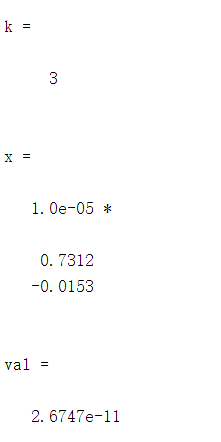
\includegraphics[width=0.8\textwidth]{newton1.png}
		%\caption{fig1}
	\end{minipage}%
}%
	\subfigure[$x_0=(1,2)^T$]{
	\begin{minipage}[t]{0.3\linewidth}
		\centering
		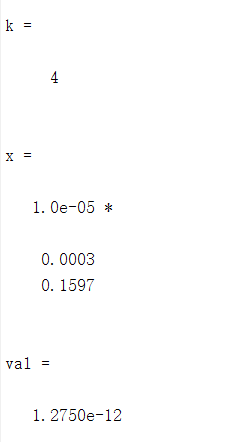
\includegraphics[width=0.8\textwidth]{newton2.png}
		%\caption{fig2}
	\end{minipage}%
}%

	\subfigure[情况一结果]{
		\begin{minipage}[t]{0.3\linewidth}
			\centering
			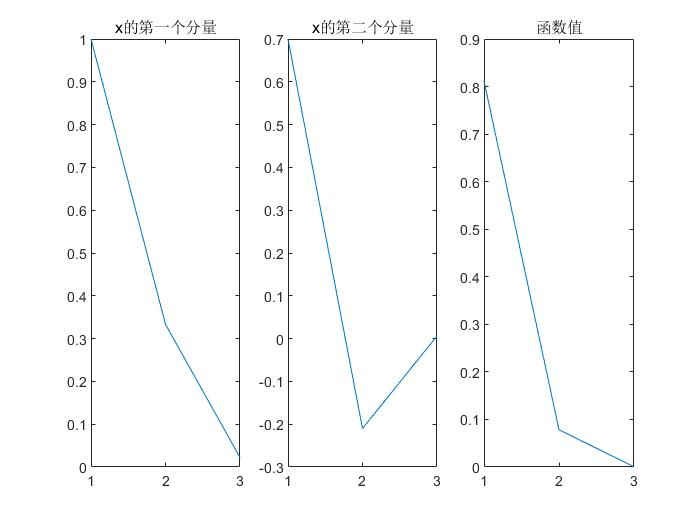
\includegraphics[width=0.8\textwidth]{nd1.jpg}
			%\caption{fig2}
		\end{minipage}
}%
	\subfigure[情况二结果]{
		\begin{minipage}[t]{0.3\linewidth}
			\centering
			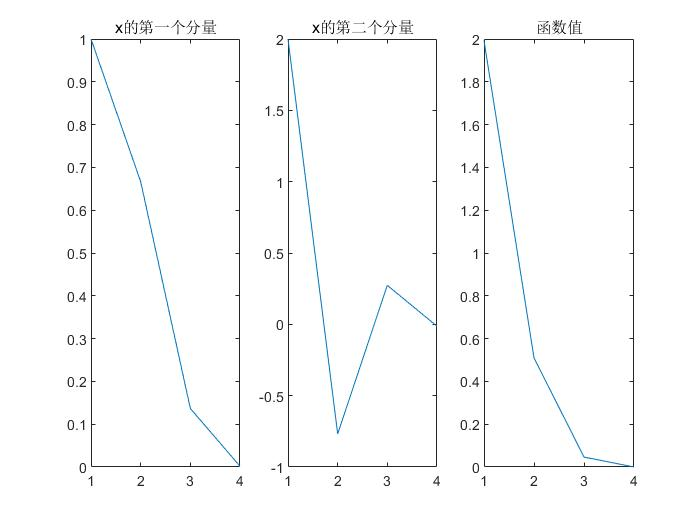
\includegraphics[width=0.8\textwidth]{nd2.jpg}
			%\caption{fig2}
		\end{minipage}
}%
	
	\centering
	\caption{基本牛顿法}
\end{figure}
	\section{牛顿型方法的数值比较}
	\subsection{线搜索程序}
	\subsubsection{精确线搜索}
	\begin{itemize}
		\item 黄金分割法
		
		输入: phi是目标函数, a, b 是搜索区间的两个端点,delta, epsilon分别是自变量和函数值的容许误差。
		
		输出: s, phis分别是近似极小点和极小值, G是nx4矩阵,其第k行分别是a,p,q,b的第k次迭代值[ak,pk,qk,bk],E=[ds,dphi], 分别是s和phis的误差限。
		
		\begin{lstlisting}
	function [s,phis,k,G,E]=golds(phi,a,b,delta,epsilon)
	t=(sqrt(5)-1)/2; h=b-a; 
	phia=feval(phi,a); phib=feval(phi,b);
	p=a+(1-t)*h;  q=a+t*h;
	phip=feval(phi,p); phiq=feval(phi,q);
	k=1;  G(k,:)=[a, p, q, b];
	while(abs(phib-phia)>epsilon)||(h>delta)
		if (phip<phiq)
			b=q;  phib=phiq; q=p; phiq=phip;
			h=b-a; p=a+(1-t)*h; phip=feval(phi,p);
		else
			a=p; phia=phip; p=q; phip=phiq;
			h=b-a;  q=a+t*h;  phiq=feval(phi,q);
		end
		k=k+1;  G(k,:)=[a, p, q, b];
	end
	ds=abs(b-a); dphi=abs(phib-phia);
	if(phip<=phiq)
		s=p;  phis=phip;
	else
		s=q;  phis=phiq;
	end
	E=[ds,dphi];
	end
		\end{lstlisting}
	\item 抛物线法
	
	输入: phi 是目标函数, a和b是搜索区间的端点,delta,epsilon是容许误差。
	
	输出: s是近似极小点, phis是对应的近似极小值; k是迭代次数,k是迭代终止时的步长, ds是|s-s1|,dphi是|phi(s1)-phi(s)|; S是迭代向量。
	\end{itemize}
	\begin{lstlisting}
	function [s,phis,k,ds,dphi,S]=qmin(phi,a,b,delta,epsilon)
	s0=a; maxj=20; maxk=30; big=1e6; err=1; k=1;
	S(k)=s0; cond=0;  h=1; ds=0.00001;
	if (abs(s0)>1e4), h=abs(s0)*(1e-4); end
	while (k<maxk && err>epsilon && cond~=5)
		f1=(feval(phi,s0+ds)-feval(phi,s0-ds))/(2*ds);
		if(f1>0), h=-abs(h); end
		s1=s0+h;     s2=s0+2*h;      bars=s0;
		phi0=feval(phi,s0);  phi1=feval(phi,s1);
		phi2=feval(phi,s2);  barphi=phi0; cond=0;
		j=0; %确定h使得phi1<phi0且phi1<phi2 
		while(j<maxj&&abs(h)>delta&&cond==0)
			if (phi0<=phi1),
				s2=s1; phi2=phi1; h=0.5*h;
				s1=s0+h; phi1=feval(phi,s1);
			else if (phi2<phi1),
				s1=s2; phi1=phi2; h=2*h;
				s2=s0+2*h; phi2=feval(phi,s2);
			else
				cond=-1; 
			end
		end
		j=j+1;
		if(abs(h)>big||abs(s0)>big), cond=5; end
	end
	if(cond==5)
		bars=s1; barphi=feval(phi,s1);
	else
		%二次插值求phis 
		d=2*(2*phi1-phi0-phi2); 
		if(d<0),
			barh=h*(4*phi1-3*phi0-phi2)/d;
		else
			barh=h/3; cond=4;
		end
		bars=s0+barh;   barphi=feval(phi,bars);
		h=abs(h);  h0=abs(barh);
		h1=abs(barh-h);  h2=abs(barh-2*h);
			%确定下一次迭代的h值
			if(h0<h), h=h0; end
			if(h1<h), h=h1; end
			if(h2<h), h=h2; end
			if(h==0), h=barh; end
			if(h<delta), cond=1; end 
			if(abs(h)>big||abs(bars)>big), cond=5; end 
			err=abs(phi1-barphi);
			s0=bars;  k=k+1; S(k)=s0;
		end
		if(cond==2 && h<delta), cond=3; end
	end
	s=s0;  phis=feval(phi,s);
	ds=abs(s-s1);  dphi=err;
	end
	\end{lstlisting}
	\subsubsection{非精确线搜索}
	\begin{itemize}
		\item Armijo准则
		
		fun和gfun分别是指目标函数及其梯度函数的子程序
		
		\begin{lstlisting}
	function [mk,alpha, newxk, fk, newfk] =armijo(xk,dk)
	beta=0.5; sigma=0.2; 
	m=0; maxm=20; 
	while (m<=maxm)
		if(fun1(xk+beta^m*dk)<=...
			fun(xk)+sigma*beta^m*gfun(xk)'*dk)
			mk=m; break; 
		end
		m=m+1;
	end
	alpha=beta^mk;
	newxk=xk+alpha*dk;
	fk=fun(xk);
	newfk=fun(newxk);
	end
		\end{lstlisting}
		\item Wolfe-Powell准则
		\begin{lstlisting}
	function [alpha, newxk, fk, newfk] = wolfe(xk, dk)
	rho = 0.25; sigma = 0.75;
	alpha = 1; a = 0; b = Inf; 
	while (1)
		if ~(fun(xk+alpha*dk)<=...
			fun(xk)+rho*alpha*gfun(xk)'*dk)
			b = alpha;
			alpha = (alpha+a)/2;
			continue;
		end
		if ~(gfun1(xk+alpha*dk)'*dk >= sigma*gfun1(xk)'*dk)
			a = alpha;
			alpha = min([2*alpha, (b+alpha)/2]);
			continue;
		end
		break;
	end
	newxk = xk+alpha*dk;
	fk = fun1(xk);
	newfk = fun1(newxk);
		\end{lstlisting}
	\end{itemize}
	\subsection{阻尼牛顿法和修正牛顿法程序}
	\begin{itemize}
		\item 阻尼牛顿法
		
		输入:fun,gfun,Hess分别是目标函数及其梯度和Hess阵,x0是初始点,epsilon为容许误差。
		
		输出:k是迭代次数,x,val分别是近似最优点和最优值。
	\begin{lstlisting}
	function [k,x,val]=dampnm(fun,gfun,Hess,x0,epsilon)
	maxk=5000; 
	beta=0.5; sigma=0.4; k=0;
	while(k<maxk)
		gk=feval(gfun,x0); 
		Gk=feval(Hess,x0); 
		dk=-Gk\gk; 
		if(norm(gk)<epsilon), break; end 
			m=0; mk=0;
		while(m<20) 
			if(feval(fun,x0+beta^m*dk)...
				<=feval(fun,x0)+sigma*beta^m*gk'*dk)
				mk=m; break;
			end
			m=m+1;
		end
		x0=x0+beta^m*dk; k=k+1;
	end
	x=x0;
	val=feval(fun,x);
	end
	\end{lstlisting}
		\item 修正牛顿法
		
		输入:fun,gfun,Hess分别是目标函数及其梯度和Hess阵,x0是初始点,epsilon为容许误差。
		
		输出:k是迭代次数,x,val分别是近似最优点和最优值。
		\begin{lstlisting}
	function [k,x,val]=revisenm(fun,gfun,Hess,x0,epsilon)
	n=length(x0); maxk=5000; 
	beta=0.5; sigma=0.4; tau=0.0; k=0; 
	while(k<maxk)
		gk=feval(gfun,x0);
		muk=norm(gk)^(1+tau);
		Gk=feval(Hess,x0);
		Ak=Gk+muk*eye(n);
		dk=-Ak\gk;
		if(norm(gk)<epsilon), break; end 
		m=0; mk=0; 
		while(m<20)
			if(feval(fun,x0+beta^m*dk)...
				<=feval(fun,x0)+sigma*beta^m*gk'*dk) 
				mk=m; break;
			end
			m=m+1;
		end
		x0=x0+beta^mk*dk;
		k=k+1;
	end
	x=x0;
	val=feval(fun,x);
	end
		\end{lstlisting}	
	\end{itemize}
	\subsection{对称秩1、BFGS、DFP算法程序}
	\begin{itemize}
		\item 对称秩1算法
		
		输入: fun,gfun分别是目标函数及其梯度,$x_0$是初始点,epsilon是容许误差,N是最大迭代次数。
		
		输出:k是迭代次数,x,val分别是近似最优点和最优值。
		\begin{lstlisting}
	function [k,x,val] = sr1(fun,gfun,x0,epsilon,N)
	if nargin<5, N=1000; end
	if nargin<4, epsilon=1.e-5; end
	beta=0.55; sigma=0.4;
	n=length(x0); Hk=eye(n); k=0;
	while(k<N)
		gk=feval(gfun,x0);
		dk=-Hk*gk;
		if(norm(gk)<epsilon), break; end 
		m=0; mk=0;
		while(m<20)
			if(feval(fun,x0+beta^m*dk)<=feval(fun,x0)...
				+sigma*beta^m*gk'*dk)
				mk=m; break;
			end
			m=m+1;
		end
		x=x0+beta^mk*dk;
		sk=x-x0; yk=feval(gfun,x)-gk;
		Hk=Hk+(sk-Hk*yk)*(sk-Hk*yk)'/((sk-Hk*yk)'*yk);
		k=k+1; x0=x;
	end
	val=feval(fun,x0);
	end
		\end{lstlisting}
	\item BFGS算法
	
	输入: fun,gfun分别是目标函数及其梯度,$x_0$是初始点,varargin是输入的可变参数变量,简单调用BFGS是可以忽略的。
	
	输出:k是迭代次数,x,val分别是近似最优点和最优值。
	\begin{lstlisting}
	function [k,x,val] = bfgs(fun,gfun,x0,varargin)
	N=1000;
	epsilon=1.e-5;
	beta=0.55; sigma=0.4;
	n=length(x0); Bk=eye(n);
	k=0;
	while(k<N)
		gk=feval(gfun,x0,varargin{:});
		if(norm(gk)<epsilon), break; end 
		dk=-Bk\gk;
		m=0; mk=0;
		while(m<20)
			newf=feval(fun,x0+beta^m*dk,varargin{:});
			oldf=feval(fun,x0,varargin{:});
			if(newf<=oldf+sigma*beta^m*gk'*dk)
				mk=m; break;
			end
			m=m+1;
		end
		x=x0+beta^mk*dk;
		sk=x-x0;
		yk=feval(gfun,x,varargin{:})-gk;
		if(yk'*sk>0)
			Bk=Bk-(Bk*sk*sk'*Bk)/(sk'*Bk*sk)+(yk*yk')/(yk'*sk);
		end
		k=k+1;
		x0=x;
	end
	val=feval(fun,x0,varargin{:});
	end
	\end{lstlisting}
	\item DFP算法
	
	输入: fun,gfun分别是目标函数及其梯度,$x_0$是初始点,epsilon是容许误差,N是最大迭代次数。
	
	输出:k是迭代次数,x,val分别是近似最优点和最优值。
	\begin{lstlisting}
	function [k,x,val] = dfp(fun,gfun,x0,epsilon,N)
	if nargin<5, N=1000; end
	if nargin<4, epsilon=1.e-5; end
	beta=0.55; sigma=0.4;
	n=length(x0); Hk=eye(n); k=0;
	while(k<N)
	gk=feval(gfun,x0);
	if(norm(gk)<epsilon), break; end
	dk=-Hk*gk;
	m=0; mk=0;
	while(m<20)
		if(feval(fun,x0+beta^m*dk)<=feval(fun,x0)...
			+sigma*beta^m*gk'*dk)
			mk=m; break;
		end
		m=m+1;
	end
	x=x0+beta^mk*dk;
	sk=x-x0; yk=feval(gfun,x)-gk;
	if(sk'*yk>0)
		Hk=Hk-(Hk*yk*yk'*Hk)/(yk'*Hk*yk)+(sk*sk')/(sk'*yk);
	end
	k=k+1; x0=x;
	end
	val=feval(fun,x0);
	end
	\end{lstlisting}
	\end{itemize}
	\subsection{问题求解}
	\begin{gather*}
	min\sum_{i=1}^{m}r_i^2(x)
	\end{gather*}
	\subsubsection{Watson函数}
	\begin{gather*}
	r_i(x)=\sum_{j=2}^{N} (j-1)x_jt_i^{j-2}-(\sum_{j=1}^{N} x_jt_i^{j-1})^2-1\\
	t_i=\frac{i}{29},1\le i\le 29\\
	r_{30}(x)=x_1\\
	r_{31}(x)=x_2-x_1^2-1\\
	2\le n\le31,m=31\\
	x_0=(0,\ldots,0)^T
	\end{gather*}
	
	构建fun2.m、gfun2.m函数
	\begin{lstlisting}
	%%目标函数
	function F=fun2(x)
	F=0;
	n=length(x);ff=0;t=(1:29)/29;
	f(30)=x(1);
	f(31)=x(2)-x(1)^2-1;
	for i = 1:29
		for j = 2:n
			f(i)=f(i)+(j-1)*x(j)*t(i)^(j-2);
		end
		for k = 1:n
			ff=ff+x(k)*t(i)^(k-1);
		end
		f(i)=f(i)-ff^2-1;
		F=F+f(i)^2;
	end
	F=F+f(30)^2+f(31)^2;
	end
	%%梯度
	function gf=gfun2(x)
	n=length(x);
	y=sym('x',[1,n]);
	gf=vpa(zeros(n,1));
	for i=1:n
		syms (['x',num2str(i)]);    
	end
	for j = 1:n
		gf(j)=diff(fun2(y),y(j));
	end
	for k = 1:n
		for m = 1:n
			gf(k)=subs(gf(k),x(m));
		end
	end
	end
	%%命令行调用
	>>x0=[0;0];
	>>[k,x,val]=sr1('fun2','gfun2',x0);
	>>[k,x,val]=bfgs('fun2','gfun2',x0);
	>>[k,x,val]=dfp('fun2','gfun2',x0);
	\end{lstlisting}
	\subsubsection{Discre boundary value函数}
	\begin{gather*}
	r_i(x)=2x_i-x_{i-1}-x_{i+1}+h^2\frac{(x_i+t_i+1)^3}{2}\\
	h=\frac{1}{n+1}\\
	t_i=ih\\
	x_0=x_{n+1}=0\\
	m=n\\
	x_0=(t_1(t_1-1),\ldots,t_n(t_n-1))^T
	\end{gather*}
	
	构建fun2.m、gfun2.m函数
	\begin{lstlisting}
	%%目标函数
	function F=fun3(x)
	n=length(x);
	t=zeros(n,1);
	h=1/(n+1);F=0;
	for m = 1:n
		t(m)=m*h;
	end
	for i = 1:n
		for j = 1:n
			if j == 1 
				f(j)=2*x(j)-x(j+1)+h^2*(x(j)+t(j)+1)^3/2;
			elseif j == n
				f(j)=2*x(j)-x(j-1)+h^2*(x(j)+t(j)+1)^3/2;
			else
				f(j)=2*x(j)-x(j-1)-x(j+1)+h^2*(x(j)+t(j)+1)^3/2;
			end
		end
	F=F+f(i)^2;
	end
	end
	%%梯度
	function gf=gfun3(x)
	n=length(x);
	y=sym('x',[1,n]);
	%gf=vpa(zeros(n,1));
	for i=1:n
		syms (['x',num2str(i)]);    
	end
	for j = 1:n
		gf(j)=diff(fun3(y),y(j));
	end
	for k = 1:n
		for m = 1:n
			gf(k)=subs(gf(k),x(m));
		end
	end
	gf=gf';
	end
	%%调用函数
	n=2;t=zeros(n,1);h=1/(n+1);
	for m = 1:n
		t(m)=m*h;
	end
	for i = 1:n
		x0(i)=t(i)*(t(i)-1);
	end
	[k,x,val]=sr1('fun3','gfun3',x0);
	%[k,x,val]=bfgs('fun3','gfun3',x0);
	%[k,x,val]=dfp('fun3','gfun3',x0);
	\end{lstlisting}
	\subsection{数据可视化}
	
	考虑watson函数,同时调用sr1、bfgs、dfp函数并比较\\
	
	结果如图:
\begin{figure}[ht]
	\centering
	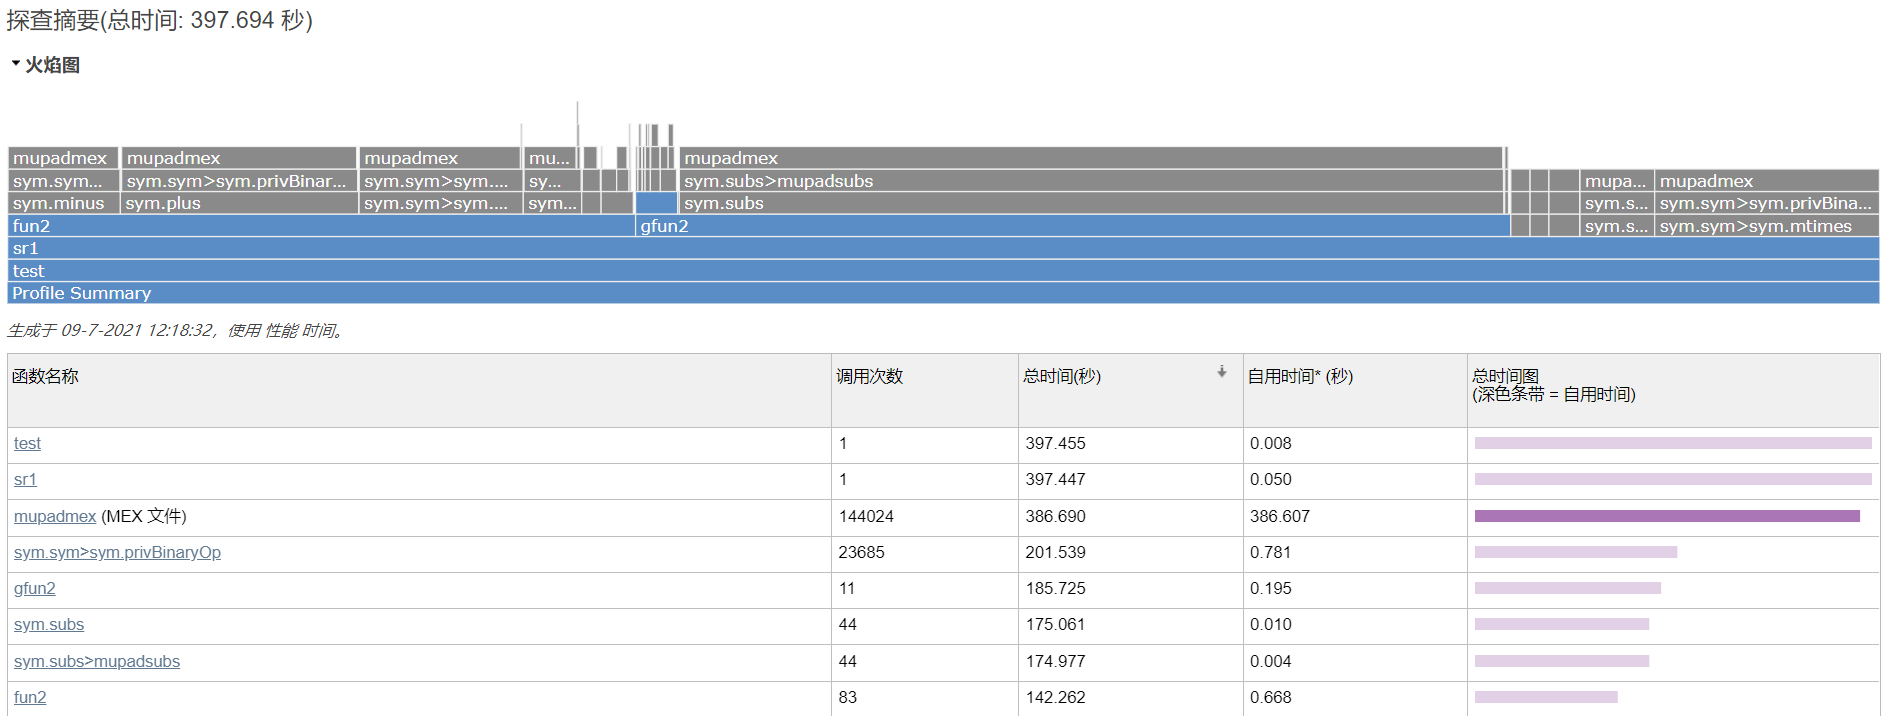
\includegraphics[width=0.65\textwidth]{sr1.png}
	\caption{sr1结果}
	\label{fig:fig1}
\end{figure}
\begin{figure}[ht]
	\centering
	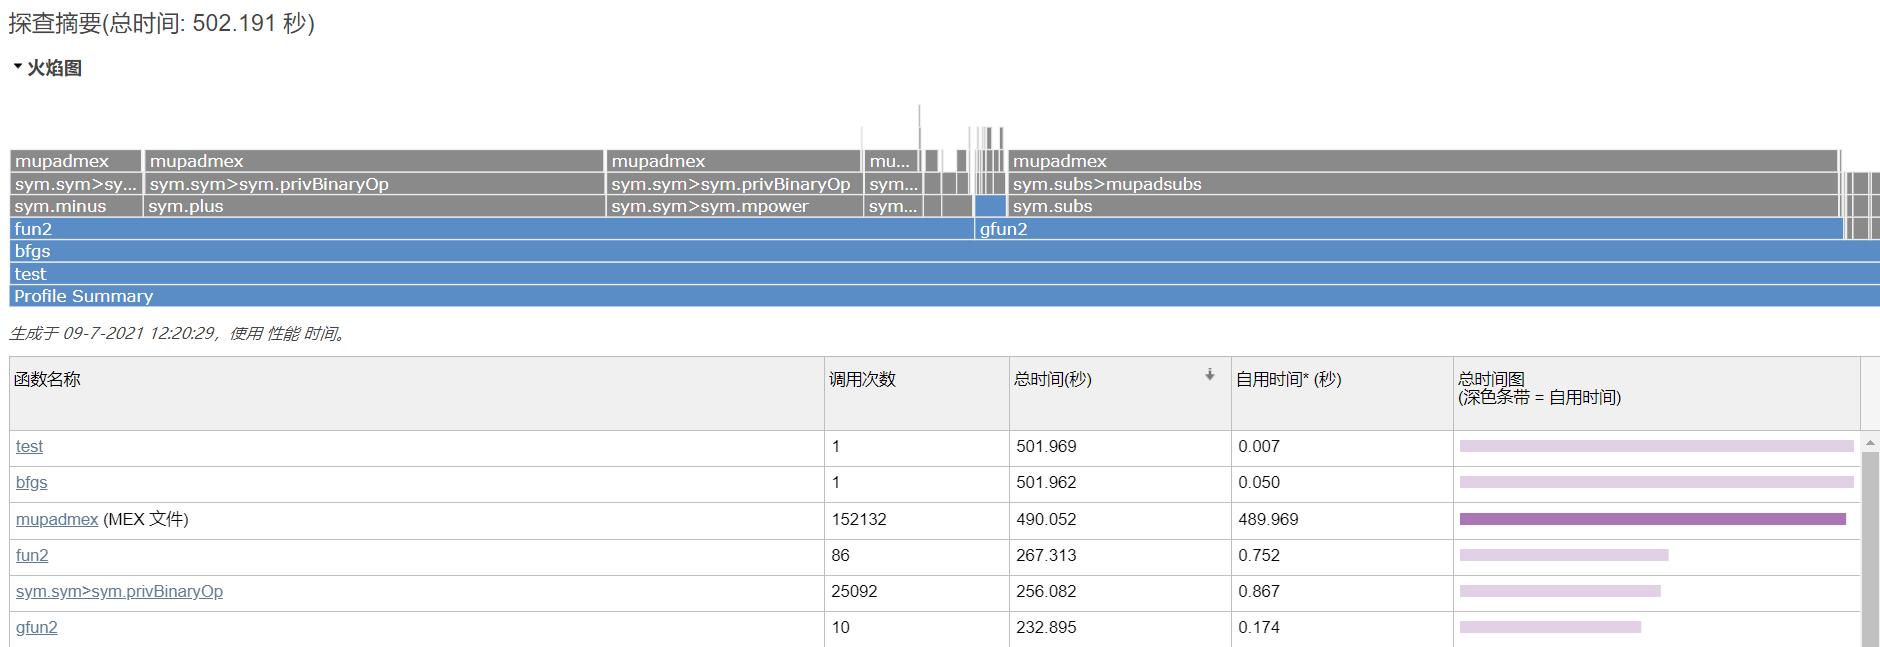
\includegraphics[width=0.65\textwidth]{bfgs1.png}
	\caption{BFGS法结果}
	\label{fig:fig1}
\end{figure}
\begin{figure}[ht]
	\centering
	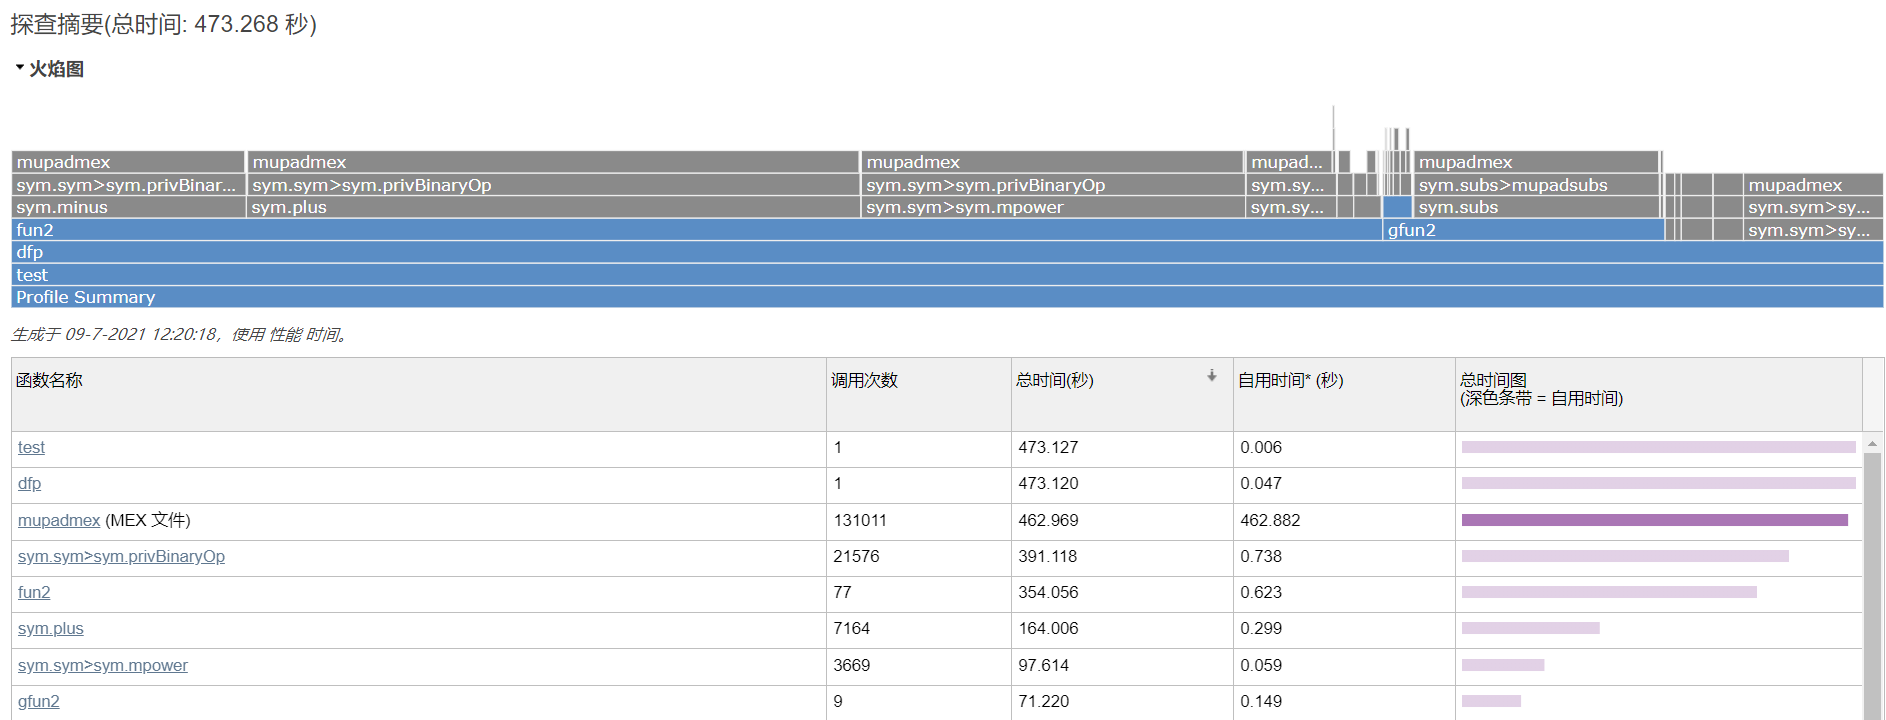
\includegraphics[width=0.65\textwidth]{dfp1.png}
	\caption{DFP法结果}
	\label{fig:fig1}
\end{figure}
	\section{梯度型算法的比较}
	\subsection{最速下降法}
			
		输入:fun,gfun分别是目标函数及其梯度,$x_0$是初始点,epsilon是容许误差。
		
		输出:k是迭代次数,x,val分别是近似最优点和最优值。
	\begin{lstlisting}
	function [k,x,val]=grad(fun,gfun,x0,epsilon)
	maxk=5000; 
	beta=0.5; sigma=0.4;
	k=0;
	while(k<maxk)
		gk=feval(gfun,x0); 
		dk=-gk;
		if(norm(gk)<epsilon), break; end 
		m=0; mk=0;
		while(m<20) 
			if(feval(fun,x0+beta^m*dk)...
				<=feval(fun,x0)+sigma*beta^m*gk'*dk)
				mk=m; break;
			end
			m=m+1;
		end
	x0=x0+beta^mk*dk;
	k=k+1;
	end
	x=x0; val=feval(fun,x0);
	end
	\end{lstlisting}
	\subsection{共轭梯度法}
	
	以FR非线性共轭梯度法为例
	
	输入:fun,gfun分别是目标函数及其梯度,$x_0$是初始点,epsilon是容许误差,N是最大迭代次数。
	\begin{lstlisting}
	function [k,x,val] = frcg(fun,gfun,x0,epsilon,N)
	if nargin<5, N=1000; end
	if nargin<4, epsilon=1.e-5; end
	beta=0.6; sigma=0.4;
	n=length(x0); k=0;
	while(k<N)
		gk=feval(gfun,x0); 
		itern=k-(n+1)*floor(k/(n+1));
		itern=itern+1;
		if(itern==1)
			dk=-gk;
		else
			betak=(gk'*gk)/(g0'*g0);
			dk=-gk+betak*d0; gd=gk'*dk;
			if(gd>=0.0), dk=-gk; end
		end
		if(norm(gk)<epsilon), break; end
		m=0; mk=0;
		while(m<20) 
			if(feval(fun,x0+beta^m*dk)...
				<=feval(fun,x0)+sigma*beta^m*gk'*dk)
				mk=m; break;
			end
			m=m+1;
		end
		x=x0+beta^mk*dk;
		g0=gk; d0=dk;
		x0=x;  k=k+1;
	end
	val=feval(fun,x);
	end
	\end{lstlisting}
	\subsection{问题求解}
	\begin{gather*}
		min\quad f(x)=4x_1^2+4x_2^2-4x_1x_2-12x_2\\
		x_0=(-0.5,1)^T
	\end{gather*}
	
	答:建立目标函数fun.m及其梯度gfun.m
	\begin{lstlisting}
	%%目标函数
	function f=fun(x)
	f=4*x(1)^2+4*x(2)^2-4*x(1)*x(2)-12*x(2);
	end
	%%梯度
	function gf=gfun(x)
	gf=[8*x(1)-4*x(2);8*x(2)-4*x(1)-12];
	end
	\end{lstlisting}
	\begin{itemize}
	\item 调用最速下降法
	\begin{lstlisting}
	>> x0=[-0.5;1];
	>> [k,x,val]=grad('fun','gfun',x0,1e-5)
	\end{lstlisting}
	
	结果如下:
	\begin{figure}[ht]
		\centering
		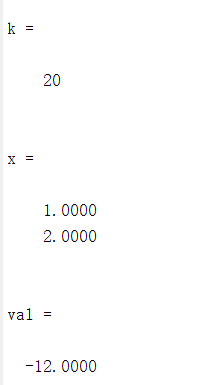
\includegraphics[width=0.2\textwidth]{zuisu.png}
		\caption{question4:最速下降法结果}
		\label{fig:fig1}
	\end{figure}
	\item 调用共轭梯度法
	\begin{lstlisting}
	>> x0=[-0.5;1];
	>> [k,x,val]=frcg('fun','gfun',x0)
	\end{lstlisting}
	
	结果如下:
	\begin{figure}[ht]
	\centering
	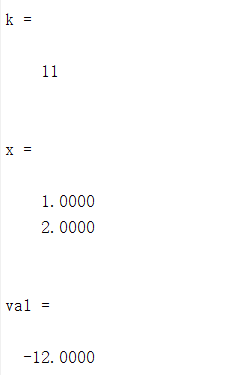
\includegraphics[width=0.25\textwidth]{gonge.png}
	\caption{question4:最速下降法结果}
	\label{fig:fig1}
	\end{figure}
	\item \textcolor{red}{分析:}共轭梯度法迭代速度较快
	\end{itemize}
	\section{非线性最小二乘问题的求解算法的比较}
	\subsection{Gauss-Newton方法}

	输入:Fk,JFk分别是求$F(x_k)$及$F'(x_k)$的函数,$x_0$是初始点,epsilon是容许误差,N是最大迭代次数。

	输出:k是迭代次数,x,val分别是近似解及$||F(x_k)||$的值。
	\begin{lstlisting}
	function [k,x,val] = gmm(Fk,JFk,x0,epsilon,N)
	if nargin<5, N=1000; end
	if nargin<4, epsilon=1.e-5; end
	beta=0.55; sigma=0.4;
	k=0;
	while(k<N)
		fk=feval(Fk,x0);
		jfk=feval(JFk,x0);
		gk=jfk'*fk; dk=-(jfk'*jfk)\gk;
		if(norm(gk)<epsilon), break; end
		m=0; mk=0;
		while(m<20)
			fnew=0.5*norm(feval(Fk,x0+beta^m*dk))^2;
			fold=0.5*norm(feval(Fk,x0))^2;
			if(fnew<fold+sigma*beta^m*gk'*dk)
				mk=m; break;
			end
			m=m+1;
		end
		x0=x0+beta^mk*dk;
		muk=norm(feval(Fk,x0));
		k=k+1;
	end
	x=x0;
	val=0.5*muk^2;
	end
	\end{lstlisting}
	\subsection{Levenberg-Marquardt方法}
	
	输入:Fk,JFk分别是求$F(x_k)$及$F'(x_k)$的函数,$x_0$是初始点,epsilon是容许误差,N是最大迭代次数。
	
	输出:k是迭代次数,x,val分别是近似解及$||F(x_k)||$的值。
	
	\begin{lstlisting}
	function [k,x,val] = lmm(Fk,JFk,x0,epsilon,N)
	if nargin<5, N=1000; end
	if nargin<4, epsilon=1.e-5; end
	beta=0.55; sigma=0.4;
	n=length(x0);
	muk=norm(feval(Fk,x0));
	k=0;
	while(k<N)
		fk=feval(Fk,x0);
		jfk=feval(JFk,x0);
		gk=jfk'*fk; dk=-(jfk'*jfk+muk*eye(n))\gk;
		if(norm(gk)<epsilon), break; end
		m=0; mk=0;
		while(m<20)
			fnew=0.5*norm(feval(Fk,x0+beta^m*dk))^2;
			fold=0.5*norm(feval(Fk,x0))^2;
			if(fnew<fold+sigma*beta^m*gk'*dk)
				mk=m; break;
			end
			m=m+1;
		end
		x0=x0+beta^mk*dk;
		muk=norm(feval(Fk,x0));
		k=k+1;
	end
	x=x0;
	val=0.5*muk^2;
	end
	\end{lstlisting}
	\subsection{问题求解}、
	
	由于Gauss-Newton算法在迭代过程中要求矩阵$J(x_k)$列满秩,这一问题在Levenberg-Marquardt方法中得到改进,这说明L-M方法的有效性优于G-N法,于是下述问题采用L-M方法。
	\subsubsection{问题1}
	\begin{gather*}
	minf(x)=\frac{1}{2}\sum_{i=1}^{5} r_i(x)^2\\
	r_1(x)=x_1^2+x_2^2+x_3^2-1\\
	r_2(x)=x_1+x_2+x_3-1\\
	r_3(x)=x_1^2+x_2^2+(x_3-2)^2-1\\
	r_4(x)=x_1+x_2-x_3+1\\
	r_5(x)=x_1^3+3x_2^2+(5x_3-x_1+1)^2-36t\\
	if\quad t=1,x^*=(0,0,1)^T
	\end{gather*}
	
	构建目标函数Fk.m及其梯度Jfk.m
	\begin{lstlisting}
	%%目标函数
	function F=Fk(x)
	F=zeros(5,1);
	t=1;%t可能为0.5或5
	F(1)=x(1)^2+x(2)^2+x(3)^2-1;
	F(2)=x(1)+x(2)+x(3)-1;
	F(3)=x(1)^2+x(2)^2+(x(3)-2)^2-1;
	F(4)=x(1)+x(2)-x(3)+1;
	F(5)=x(1)^3+3*x(2)^2+(5*x(3)-x(1)+1)^2-36*t;
	end
	%%梯度
	function JF = JFk(x)
	JF=[2*x(1),2*x(2),2*x(3);
	1,1,1;
	2*x(1),2*x(2),2*(x(3)-2);
	1,1,-1;
	3*x(1)^2-2*(5*x(3)-x(1)+1),6*x(2),10*(5*x(3)-x(1)+1)];
	end
	\end{lstlisting}
	
	结果如下:
	\begin{figure}[ht]
		\centering
		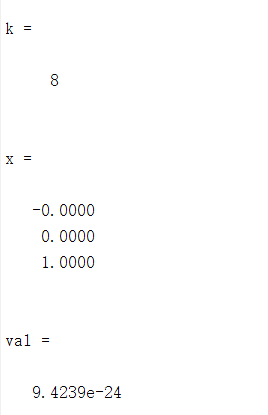
\includegraphics[width=0.35\textwidth]{gmm1.png}
		\caption{question5:t=1时}
		\label{fig:fig1}
	\end{figure}
	
	t=0.5或t=5时结果如下:
	\begin{figure}[htbp]
		\centering
		
		\subfigure[t=0.5]{
			\begin{minipage}[t]{0.35\linewidth}
				\centering
				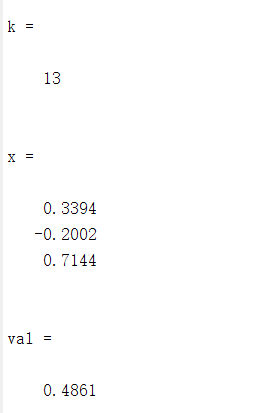
\includegraphics[width=0.7\textwidth]{gmm2.png}
				%\caption{fig1}
			\end{minipage}%
		}%
		\subfigure[t=5]{
			\begin{minipage}[t]{0.35\linewidth}
				\centering
				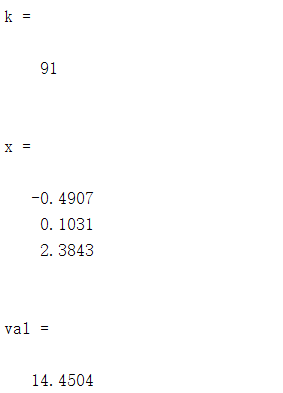
\includegraphics[width=0.7\textwidth]{gmm3.png}
				%\caption{fig2}
			\end{minipage}%
		}%
		%这个回车键很重要 \quad也可以
		\centering
		\caption{question5:t为其他情况}
	\end{figure}
	\subsubsection{问题2:扩展Rosenbrock问题}
	\begin{gather*}
	minf(x)=\frac{1}{2}\sum_{i=1}^{m} r_i(x)^2\\
	r_{2i+1}(x)=10(x_{2i}-x_{2i-1}^2)\\
	r_{2i}(x)=1-x_{2i-1}\\
	x\in R^n,n=2k(k\in N),m=n\\
	x^*=(1,\ldots,1)^T,f^*=0\\
	x^{(0)}=(x_1^{(0)},\ldots,x_n^{(0)})\\
	x_{2j-1}^{(0)}=-1.2,x_{2j}^{(0)}=1
	\end{gather*}
	
	构建目标函数Fk2.m及其梯度Jfk2.m
	\begin{lstlisting}
	%%目标函数
	function F=Fk2(x)
	n=length(x);F=zeros(n,1);
	for i =1:n
		if ~mod(i,2)
			F(i)=1-x(i-1);
		elseif mod(i,2)
			F(i)=10*(x(i+1)-x(i)^2);
		end
	end
	end
	%%梯度
	function JF=JFk2(x)
	n=length(x); JF=zeros(n,n);
	for i=1:n
		for j= 1:n
			if i==j && ~mod(j,2)
				JF(i,j)=0;
			elseif i==j && mod(j,2)
				JF(i,j)=-20*x(i);
			end
			if (i-j)==1 && ~mod(j,2)
				JF(i,j)=0;
			elseif (i-j)==1 && mod(j,2)
				JF(i,j)=-1;
			end
			if (j-i)==1 && ~mod(i,2)
				JF(i,j)=0;
			elseif (j-i)==1 && mod(i,2)
				JF(i,j)=10;
			end
		end
	end
	%%命令窗口
	>> n=10;
	>> x0=x0(n);
	>> [k,x,val] = gmm('Fk2','JFk2',x0)
	\end{lstlisting}
	
	结果如下图:
	\begin{figure}[ht]
		\centering
		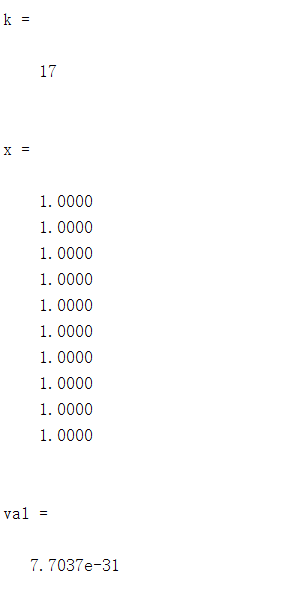
\includegraphics[width=0.4\textwidth]{rosen.png}
		\caption{question5:Rosenbrock结果}
		\label{fig:fig1}
	\end{figure}
	\section{约束优化问题的罚函数算法的比较}
	\subsection{外点罚函数法求解}
	\begin{gather*}
	min f(x)=ln(1+x_1^2)-x_2\\
	s.t.\quad (1+x_1^2)^2+x_2^2-4=0\\
	x_0=(2,2)^T\\
	x^*=(0,\sqrt{3})^T,f(x^*)=-\sqrt{3}
	\end{gather*}
	
	构建下列函数:
	\begin{itemize}
	\item 目标函数obj.m
	\item 约束条件函数constrains.m
	\item 增广目标函数Al obj.m
	\item 罚函数compare.m
	\item 罚函数求解函数Al main.m
	\end{itemize}
\begin{lstlisting}
	%%目标函数
	function f=obj(x)
	f=log(1+x(1)^2)-x(2);
	end
	%%约束条件函数
	function [h,g]=constrains(x)
	h=(1+x(1)^2)^2+x(2)^2-4;
	end
	%%增广目标函数
	function f=AL_obj(x)
	global pena N_equ;
	h_equ=0;
	h_inequ=0;
	h=constrains(x);
	for i=1:N_equ
		h_equ=h_equ+h(i).^2;
	end
	f=obj(x)+pena*(h_equ+h_inequ);
	end
	%%罚函数
	function f=compare(x)
	global pena N_equ;
	h_equ=0;
	h_inequ=0;
	h=constrains(x);
	for i=1:N_equ
		h_equ=h_equ+h(i).^2;
	end
	f=pena*(h_equ+h_inequ);
	end
	%%罚函数求解函数
	function [X,FVAL]=AL_main(x_al,N_equ,N_inequ)
	global pena N_equ;
	pena=0.1;
	c_scale=2;
	e_al=1e-6;
	max_itera=100;
	out_itera=1;
	while out_itera<max_itera
		x_al0=x_al;
		[X,FVAL]=fminunc(@AL_obj,x_al0);
		x_al=X;
		if compare(x_al)<=e_al
			break;
		end
		pena=c_scale*pena;
		out_itera=out_itera+1;
	end
	X=x_al;
	FVAL=obj(X);
	end
\end{lstlisting}

	结果如下:
	\begin{figure}[ht]
		\centering
		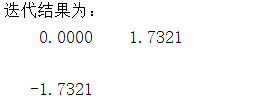
\includegraphics[width=0.35\textwidth]{waidian.png}
		\caption{question6:外点罚函数法}
		\label{fig:fig1}
	\end{figure}

\textcolor{red}{分析:外点法对此问题有效}
	\subsection{内点罚函数法求解}
	\begin{gather*}
	min f(x)=-x_1x_2x_3\\
	s.t.\quad -{x_1}^2-2{x_2}^2-4{x_3}^2+48\ge0\\
	x_0=(1,1,1)\\
	x^*=(a,b,c)^T,(a,-b,-c)^T,(-a,b,-c)^T,(-a,-b,c)^T,f(x^*)=-16\sqrt{2}\\
	a=4,b=2\sqrt{2},c=2
	\end{gather*}
	
	构建下述Matlab文件
\begin{itemize}
	\item 目标函数obj.m
	\item 约束条件函数constrains.m
	\item 增广目标函数Al obj.m
	\item 罚函数compare.m
	\item 罚函数求解函数Al main.m
\end{itemize}
\begin{lstlisting}
	%%
	function f=obj(x)
	f=-(x(1)*x(2)*x(3));;
	end
	%%
	function [h,g]=constrains(x)
	g=-x(1)^2-2*x(2)^2-4*x(3)^2+48;
	end
	%%
	function f=AL_obj(x)
	global pena N_inequ;
	h_inequ=0;
	g=constrains(x);
	for i=1:N_inequ
		h_inequ=h_inequ-log(g(i));
	end
	f=obj(x)+pena*(h_inequ);
	end
	%%
	function f=compare(x)
	global pena N_inequ;
	h_inequ=0;
	g=constrains(x);
	for i=1:N_inequ
		h_inequ=h_inequ-log(g(i));
	end
	f=pena*(h_inequ);
	end
	%%
	function [X,FVAL]=AL_main(x_al,N_equ,N_inequ)
	global pena N_equ N_inequ;
	pena=10;
	c_scale=0.5;
	e_al=1e-6;
	max_itera=100;
	out_itera=1;
	while out_itera<max_itera
		x_al0=x_al;
		[X,FVAL]=fminunc(@AL_obj,x_al0);
		x_al=X;
		if compare(x_al)<=e_al
			break;
		end
		pena=c_scale*pena;
		out_itera=out_itera+1;
	end
	X=x_al;
	FVAL=obj(X);
	end
\end{lstlisting}

构建main.m输入参数求解
\begin{lstlisting}
	function main()
	clc,clear;
	x_al=[4,2*sqrt(2),2];
	N_inequ=1;
	[X,FVAL]=AL_main(x_al,N_inequ);
	disp(X);disp(FVAL);
	end
\end{lstlisting}

结果如下
\begin{figure}[ht]
	\centering
	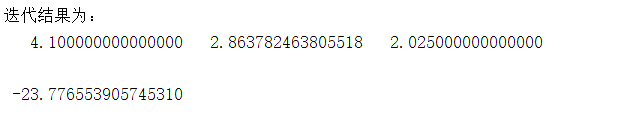
\includegraphics[width=0.8\textwidth]{neidian.png}
	\caption{内点罚函数法结果}
	\label{fig:fig1}
	\textcolor{red}{分析:当初值为$x_0=(1,1,1)^T$时,内点法结果不为最优解,而当初值足够靠近最优解时,解也足够靠近最优值,说明对此问题,内点法有效性较差}
\end{figure}
	\subsection{乘子法求解}
	\begin{gather*}
	min f(x)=(x_1-1)^2+(x_1-x_2)^2+(x_2-x_3)^2\\
	s.t.\quad x_1(1+{x_2}^2)+{x_3}^4-4-3\sqrt{2}\\
	-10\le x_i\le10,i=1,2,3\\
	x_0=(2,2,2)^T\\
	x^*=(1.104859024,1.196674194,1.535262257)^T,f(x^*)=0.03256820025
	\end{gather*}
	
	构建下述Matlab文件
	\begin{itemize}
		\item PHR算法函数multphr.m
		\item 增广拉格朗日函数mpsi.m
		\item 增广拉格朗日函数的梯度dmpsi.m
		\item 目标函数f1.m
		\item 等式约束函数h1.m
		\item 不等式约束函数g1.m
		\item 目标函数的梯度df1.m
		\item 等式约束的Jacob矩阵转置dh1.m
		\item 不等式约束的Jacob矩阵转置dg1.m
	\end{itemize}
	\begin{lstlisting}
	%%
	function [x,mu,lam,output]=multphr(fun,hf,gf,dfun,dhf,dgf,x0)
	maxk=1000;  %最大迭代次数
	sigma=2.0;  %罚因子
	theta=0.8;  eta=2.0;  %PHR算法中的实参数
	k=0;  ink=0;  %k,ink分别是外迭代和内迭代次数
	epsilon=1e-5;  %终止误差值
	x=x0;  he=feval(hf,x);  gi=feval(gf,x);
	n=length(x);  l=length(he);  m=length(gi);
	%选取乘子向量的初始值
	mu=0.1*ones(l,1);  lam=0.1*ones(m,1);
	betak=10;  betaold=10;  %用来检验终止条件的两个值
	while(betak>epsilon && k<maxk)
		%调用BFGS算法程序求解无约束子问题
		[ik,x,val]=bfgs('mpsi','dmpsi',x0,fun,hf,gf,dfun,...
		dhf,dgf,mu,lam,sigma);
		ink=ink+ik;
		he=feval(hf,x); gi=feval(gf,x);
		%计算batak
		betak=sqrt(norm(he,2)^2+norm(min(gi,lam/sigma),2)^2);
		if betak>epsilon
			%更新乘子向量
			mu=mu-sigma*he;
			lam=max(0.0,lam-sigma*gi);
			if(k>=2 && betak>theta*betaold)
				sigma=eta*sigma;
			end
		end
		k=k+1;
		betaold=betak;
		x0=x;
	end
	f=feval(fun,x);
	output.fval=f;
	output.iter=k;
	output.inner_iter=ink;
	output.beta=betak;
	%%
	function psi=mpsi(x,fun,hf,gf,dfun,dhf,dgf,mu,lam,sigma)
	f=feval(fun,x);  he=feval(hf,x);  gi=feval(gf,x);
	l=length(he);  m=length(gi);
	psi=f;  s1=0.0;
	for i=1:l
		psi=psi-he(i)*mu(i);
		s1=s1+he(i)^2;
	end
	psi=psi+0.5*sigma*s1;
	s2=0.0;
	for i=1:m
		s3=max(0.0,lam(i)-sigma*gi(i));
		s2=s2+s3^2-lam(i)^2;
	end
	psi=psi+s2/(2.0*sigma);
	end
	%%
	function dpsi=dmpsi(x,fun,hf,gf,dfun,dhf,dgf,mu,lam,sigma)
	dpsi=feval(dfun,x);
	he=feval(hf,x);  gi=feval(gf,x);
	dhe=feval(dhf,x);  dgi=feval(dgf,x);
	l=length(he);  m=length(gi);
	for i=1:l
		dpsi=dpsi+(sigma*he(i)-mu(i))*dhe(:,i);
	end
	for i=1:m
		dpsi=dpsi+(sigma*gi(i)-lam(i))*dgi(:,i);
	end
	end
	%%
	function f=f1(x)
	f=(x(1)-1)^2+(x(1)-x(2))^2+(x(2)-x(3))^4;
	end
	%%
	function he=h1(x)
	he=x(1)*(1+x(2)^2)+x(3)^4-4-3*sqrt(2);
	end    
	%%
	function gi=g1(x)
	gi=[x(1)+10;
	x(2)+10;
	x(3)+10;
	-x(1)+10;
	-x(2)+10;
	-x(3)+10;];
	end
	%%
	function g=df1(x)
	g=[4*x(1)-2*x(2)-2;
	2*x(2)-2*x(1)+4*(x(2)-x(3))^3;
	-4*(x(2)-x(3))^3]; 
	end
	%%
	function dhe=dh1(x)
	dhe=[x(2)^2+1,2*x(1)*x(2),4*x(3)^3]';
	end
	%%
	function dgi=dg1(x)
	dgi=[eye(3);-1*eye(3)]';
	end
	\end{lstlisting}
	
	命令窗口输入:
	\begin{lstlisting}
	x0=[2,2,2]';
	[x,mu,lam,output]=multphr('f1','h1','g1','df1','dh1','dg1',x0)
	\end{lstlisting}

结果如下
\begin{figure}[ht]
	\centering
	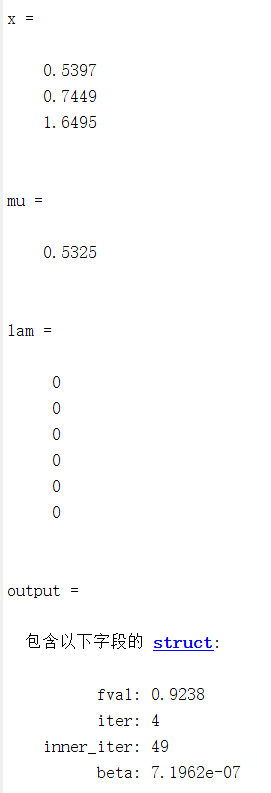
\includegraphics[width=0.25\textwidth]{chengzi.png}
	\caption{乘子法结果}
	\label{fig:fig1}
\end{figure}
\begin{figure}[ht]
	\centering
	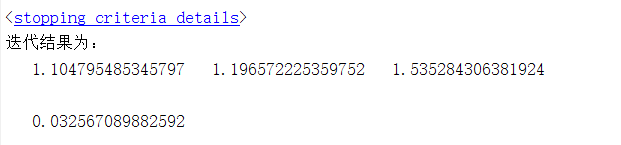
\includegraphics[width=0.45\textwidth]{waidian2.png}
	\caption{外点法结果}
	\label{fig:fig1}
\end{figure}

\textcolor{red}{分析:由结果可知,乘子法对此问题有效性很差,而不难验证,使用本题第一问外点法(修改函数)求解此题,结果正确,但初始点却为可行点}
\end{document}